% SPAR Midterm Report - LLM Forecaster Variance Analysis
% This section follows Jeff's Methods section on forecast elicitation and consistency metrics
% Compatible with arXiv (TeX Live 2023+, pdflatex)

\documentclass[midterm]{sparreport}
\usepackage{placeins}
\usepackage{booktabs}
\usepackage{graphicx}
\usepackage{amsmath}

% ============================================================================
% METADATA
% ============================================================================
\title{Measuring Performance of LLM Forecasters for Quantitative Risk Modeling of Cyber Misuse}
\author{%
  \textbf{Jeff Author}\footnote{Placeholder - update with actual author info}\\
  \texttt{jeff@example.com}%
  \and
  \textbf{Madhav Khanal}\\
  \texttt{madhavkhanal3145@gmail.com}%
}
\sparround{Spring 2026}

\begin{document}

\maketitle

% ============================================================================
% ABSTRACT (placeholder - to be completed)
% ============================================================================
\begin{abstract}
AI-enabled cyberattacks pose significant risks from advanced AI systems. SaferAI's cybersecurity risk models use AI evaluation benchmarks to forecast capability uplift from frontier models, historically relying on expensive human expert elicitation. This project develops methodology to evaluate LLM-based automated expert elicitation as a scalable alternative. We develop consistency metrics using Wasserstein distance and Fréchet ANOVA, then probe variance sources through systematic experimental manipulation. Results show model choice explains 48--69\% of distributional variance while expert persona explains $\leq$25\%, strong baseline anchoring effects, and surprising insensitivity to prompt length. These findings inform design of reliable LLM-based forecasting systems for AI risk assessment.
\end{abstract}

\keywords{LLM evaluation \and cybersecurity risk modeling \and expert elicitation \and AI safety}

% ============================================================================
% INTRODUCTION (Jeff's section - placeholder)
% ============================================================================
\section{Introduction}

AI enabled cyberattacks are an important risk vector for advanced AI systems, and have already resulted in direct harm. SaferAI has developed 9 cybersecurity risk models that leverage AI evaluation benchmarks as key risk indicators to forecast the degree of cyberattack capabilities uplift from frontier models. Historically, the mapping between benchmark performance and forecasted uplift has relied on human expert elicitation, but this process is time consuming and expensive, which imposes limits on its utility for monitoring. SaferAI would like to use automated LLM experts to elicit these forecasts for input into risk models, allowing for scalable monitoring of a wider range of models on faster time scales, but a methodology for measuring and evaluating the capability of LLM experts at this task is currently lacking.

This project seeks to develop one such methodology, and to leverage that methodology to evaluate and improve LLM expert elicitation performance. This consists of three primary objectives. First, to develop a metric that captures desirable characteristics of elicited forecasts and can be used to compare various experimental manipulations of forecasters. Second, to use this methodology along with other statistical tools to probe the impact of various manipulations to the forecasting approach. And third, to develop an adjacent and scalable 'ground truth' accuracy that can be used to evaluate forecast quality without relying on scarce human-labelled data. This report details progress on the first two of these goals, while the third remains a future objective.

% ============================================================================
% RELATED WORK (Jeff's section - placeholder)
% ============================================================================
\section{Related Work}

Position your work relative to existing research. What prior work does your project build on? What gap does it fill? Focus on the 3--5 most relevant papers or lines of work.

% ============================================================================
% METHODS (Jeff's section - placeholder, includes forecast elicitation and consistency metrics)
% ============================================================================
\section{Methods}

\subsection{Forecast Elicitation}

The forecasts used for development in the subsequent sections are elicited using the approach described in Barret et. al 2025. Briefly, the objective of these forecasts is to estimate the probability of success on a given MITRE ATT\&CK~\cite{mitre} step conditional on observed success on a given benchmark task (taken from Cybench or BountyBench). These estimates are elicited at the modal (50\%) level, as well as 25\% and 75\% levels to give some sense of the confidence interval around this estimate.

The forecast model is complex and contains numerous features which could be experimentally manipulated. The most important components for the purposes of this report include:

\begin{itemize}
\item \textbf{Persona descriptions:} A set of custom designed prompts intended to elicit various expert perspectives during the estimation procedure. Ten distinct cybersecurity expert roles were defined (e.g., AI/ML Security Researcher, Malware Engineer, Threat Analyst).
\item \textbf{Baseline risk estimates:} Baseline values and confidence intervals for MITRE step risk taken from expert opinions. These are provided to the LLM as anchoring information.
\item \textbf{Reasoning prompts:} A chain of custom prompts instructing the forecaster on the desired forecast flow steps, including detailed analysis of provided benchmark task and guidance on reasoning steps for translating this analysis into a forecast.
\end{itemize}

\subsection{Consistency Metrics}

We quantified agreement between repeated elicitations using Wasserstein distance metrics, with the goal of developing a practical measure for evaluating subsequent modifications to the estimator. We focused on the first-order and second-order Wasserstein distances (W$_1$ and W$_2$), which summarize the discrepancy between two distributions in terms of the amount of probability mass that must be shifted to transform one distribution into the other. W$_1$ (earthmover's distance) captures the average magnitude of this shift, while W$_2$ places greater weight on larger discrepancies and is correspondingly more sensitive to occasional large deviations. Confidence intervals (95\%) were generated by bootstrapping distances across resampled sets of elicited points.

This metric serves two primary purposes:

\begin{itemize}
\item \textbf{Quantifying estimator consistency:} By comparing multiple runs with identical settings, we quantify the reliability of an estimator. Low run-to-run variability is desired, as this indicates the estimator elicits similar distributions when run with identical data.
\item \textbf{Quantifying impact of experimental modifications:} If modifying some component of the estimator (e.g., prompt components) has no impact on consistency compared to the baseline approach, it strongly suggests that this modification has minimal impact on the behavior of the estimator. This can be used to hone in on specific interventions that materially impact estimator performance.
\end{itemize}

The W$_1$ and W$_2$ metrics are primarily computed using a linear interpolation assumption, which directly compares elicited quantiles, as this removes an additional degree of uncertainty that would be introduced by fitting these points to an assumed distribution shape. In some cases, where noted, elicited points are instead fit to a beta distribution before computing the distance using numeric integration. This provides a fairer comparison for manipulations which elicit a different number of points, as the linear approach biases these comparisons towards larger distances.

In addition, we also compute discrepancy of the reported modal value and interquartile range between pairs of estimates. When aggregated, these provide a separate measure of central tendency and estimate confidence across experimental variants, which are useful summary statistics for diagnosing estimator performance.

\subsection{Fréchet ANOVA for Distributional Variance}

To test whether grouping factors (persona, model) explain distributional variance, we used Fréchet ANOVA as developed by Dubey and Müller~\cite{dubey2019frechet}: a generalization of one-way ANOVA to data in an abstract metric space. This allows us to compare $k$ groups of \emph{distributions} rather than scalar outcomes.

In our setting, each observation is a fitted Beta distribution (from elicited p25, p50, p75), distances between distributions use the $L^2$-Wasserstein metric on quantile functions, and inference follows their test construction with a permutation procedure for $p$-values. We summarize effect size with ICC\_F, the fraction of Fréchet variance attributable to the grouping factor.

\textbf{Implementation procedure:}
\begin{enumerate}
\item \textbf{Fit Beta distributions.} For each LLM response, fit Beta($\alpha$, $\beta$) from $(p_{25}, p_{50}, p_{75})$ via least squares:
$$\min_{\alpha,\beta} \sum_{q \in \{0.25, 0.50, 0.75\}} \bigl( \mathrm{CDF}(p_q; \alpha, \beta) - q \bigr)^2$$
Reject fits where $\max_q |\mathrm{CDF}(p_q) - q| > 0.05$ (internally inconsistent elicitations).

\item \textbf{Represent as quantile functions.} $Q(u) = F^{-1}(u)$, $u \in [0.001, 0.999]$, evaluated on a uniform grid of 201 points.

\item \textbf{Compute pairwise Wasserstein distances.}
$$d_W^2(F,G) = \int_0^1 \bigl(Q_F(u) - Q_G(u)\bigr)^2\, du$$
Approximated via trapezoidal integration over the quantile grid.

\item \textbf{Calculate Fréchet means.} $\bar{Q}(u) = \frac{1}{n}\sum_{i=1}^{n} Q_i(u)$, computed pointwise for each group (persona or model) and for pooled data.

\item \textbf{Calculate Fréchet variances.}
$$\hat{V}_j = \frac{1}{n_j} \sum_{i=1}^{n_j} d_W^2(Q_{ij}, \bar{Q}_j) \quad \text{(within-group)}$$
$$\hat{V}_p = \frac{1}{N} \sum_{j}\sum_{i} d_W^2(Q_{ij}, \bar{Q}_p) \quad \text{(pooled)}$$

\item \textbf{Compute test statistic $T_n$.}
$$F_n = \hat{V}_p - \sum_{j=1}^{k} \lambda_j \hat{V}_j \quad \text{(between-group variance)}$$
$$U_n = \sum_{1 \le i < j \le k} \lambda_i \lambda_j (\hat{V}_i - \hat{V}_j)^2 \quad \text{(heteroscedasticity correction)}$$
$$T_n = N \cdot F_n + N \cdot U_n$$
where $\lambda_j = n_j / N$ (group proportions).

\item \textbf{Permutation test.} Shuffle group labels 5000 times, recompute $T_n$ each time.
$$p = \frac{\#\{T_n^{\text{perm}} \ge T_n^{\text{obs}}\} + 1}{5000 + 1}$$
\end{enumerate}

% ============================================================================
% RESULTS (Madhav's main contribution)
% ============================================================================
\section{Results}

\subsection{Experimental Conditions}

All experiments varied model forecasts across the following dimensions:

\begin{itemize}
  \item \textbf{Models:} Claude Sonnet 4.5 (primary experiments), Claude Sonnet 4.6 (baseline sweep), GPT-4o, Gemini 2.5 Pro
  \item \textbf{Personas:} 10 cybersecurity expert roles evaluated within-model
  \item \textbf{Attack scenarios:} MITRE ATT\&CK steps from a ransomware scenario targeting a large enterprise. Primary steps: TA0001 (Initial Access), TA0002 (Execution), TA0007 (Discovery), T1657 (Financial Theft)
  \item \textbf{Baseline probabilities:} Three baselines tested (30\%, 50\%, 85\%) representing low, medium, and high prior success probability. Baseline sweep experiments varied from 10\% to 90\% in 10\% increments.
  \item \textbf{Benchmark tasks:} BountyBench ordered dataset. Primary task: Imaginairy (LLM-estimated difficulty = 22/100, CVSS severity = 7.5). Additional tasks: MLFlow0 (difficulty = 38, CVSS = 10.0), cURL (difficulty = 42, CVSS = 5.3).
  \item \textbf{Estimate type:} Probability (bounded 0--1) vs. quantity (number of actors, unbounded)
  \item \textbf{Prompt variations:} Seven conditions testing removal of baseline, confidence intervals, reasoning scaffolds, and capability analysis sections
\end{itemize}

All experiments used 10 runs per condition unless otherwise specified to enable robust statistical comparison.

\subsection{Model Variance Dominates Persona Variance}

\textbf{Research question:} Do different expert personas generate meaningfully different forecast distributions, or is variance primarily driven by model choice?

\textbf{Experimental design:} Fréchet ANOVA on percentile-based Beta fits. Within-model tests: 10 personas as groups, 10 runs per persona per attack step. Cross-model tests: 3 models as groups, pooling all 10 personas (100 runs per model per step). Three attack steps tested: TA0002 (50\% baseline), TA0007 (85\% baseline), T1657 (30\% baseline). All tests used Imaginairy benchmark task.

\textbf{Results:} Persona effects were weak and inconsistent. For Claude Sonnet 4.5 and GPT-4o, persona ICC\_F ranged from 5.7\% to 13.9\% with no significant effects ($p > 0.05$ for all tests, Table~\ref{tab:persona_variance}). Gemini 2.5 Pro showed two significant persona effects (max ICC\_F 24.9\%, $p < 0.05$), but these remained smaller than cross-model effects.

Cross-model comparisons showed ICC\_F of 48--69\% with all tests highly significant ($p < 0.001$, Table~\ref{tab:model_variance}), indicating model identity as the dominant variance source. Model choice explained 3.5--12$\times$ more variance than persona choice across all tested attack steps.

\begin{table}[htbp]
\centering
\caption{Within-model persona variance (Fréchet ANOVA). H$_0$: All 10 expert personas produce the same belief distribution. No significant persona effects for Claude or GPT-4o. Gemini shows limited significant variation at two steps.}
\label{tab:persona_variance}
\begin{tabular}{llcccc}
\toprule
\textbf{Model} & \textbf{Step (Baseline)} & \textbf{N} & \textbf{T$_n$} & \textbf{p-value} & \textbf{ICC\_F} \\
\midrule
\multicolumn{6}{l}{\textit{Claude Sonnet 4.5}} \\
& TA0002 (50\%) & 100 & 0.008 & 0.400 & 9.6\% \\
& TA0007 (85\%) & 80 & 0.003 & 0.195 & 13.9\% \\
& T1657 (30\%) & 100 & 0.020 & 0.803 & 7.2\% \\
\midrule
\multicolumn{6}{l}{\textit{GPT-4o}} \\
& TA0002 (50\%) & 97 & 0.016 & 0.899 & 5.7\% \\
& TA0007 (85\%) & 96 & 0.007 & 0.708 & 7.5\% \\
& T1657 (30\%) & 100 & 0.043 & 0.215 & 11.8\% \\
\midrule
\multicolumn{6}{l}{\textit{Gemini 2.5 Pro}} \\
& TA0002 (50\%) & 88 & 0.043 & \textbf{0.030} & 18.3\% \\
& TA0007 (85\%) & 96 & 0.007 & \textbf{0.002} & 24.9\% \\
& T1657 (30\%) & 88 & 0.005 & 0.585 & 8.8\% \\
\bottomrule
\end{tabular}
\end{table}

\begin{table}[htbp]
\centering
\caption{Cross-model variance (Fréchet ANOVA). H$_0$: All 3 models produce the same belief distribution. All steps show highly significant model effects. Model choice explains 48--69\% of distributional variance.}
\label{tab:model_variance}
\begin{tabular}{lcccc}
\toprule
\textbf{Step (Baseline)} & \textbf{N} & \textbf{T$_n$} & \textbf{p-value} & \textbf{ICC\_F} \\
\midrule
TA0002 (50\%) & 285 & 0.729 & <0.001 & 55.3\% \\
TA0007 (85\%) & 272 & 0.131 & <0.001 & 48.2\% \\
T1657 (30\%) & 288 & 1.515 & <0.001 & 69.4\% \\
\bottomrule
\end{tabular}
\end{table}

Visualizations confirm these patterns. Figure~\ref{fig:persona_dist} shows persona distributions overlapping tightly within each model-step combination for Claude Sonnet 4.5, while Figure~\ref{fig:model_dist} shows clear separation between models across all three attack steps. Figure~\ref{fig:full_grid} displays the full experimental grid across all models, attack steps, and personas, showing within-cell persona clustering is much tighter than between-model shifts.

\begin{figure}[htbp]
  \centering
  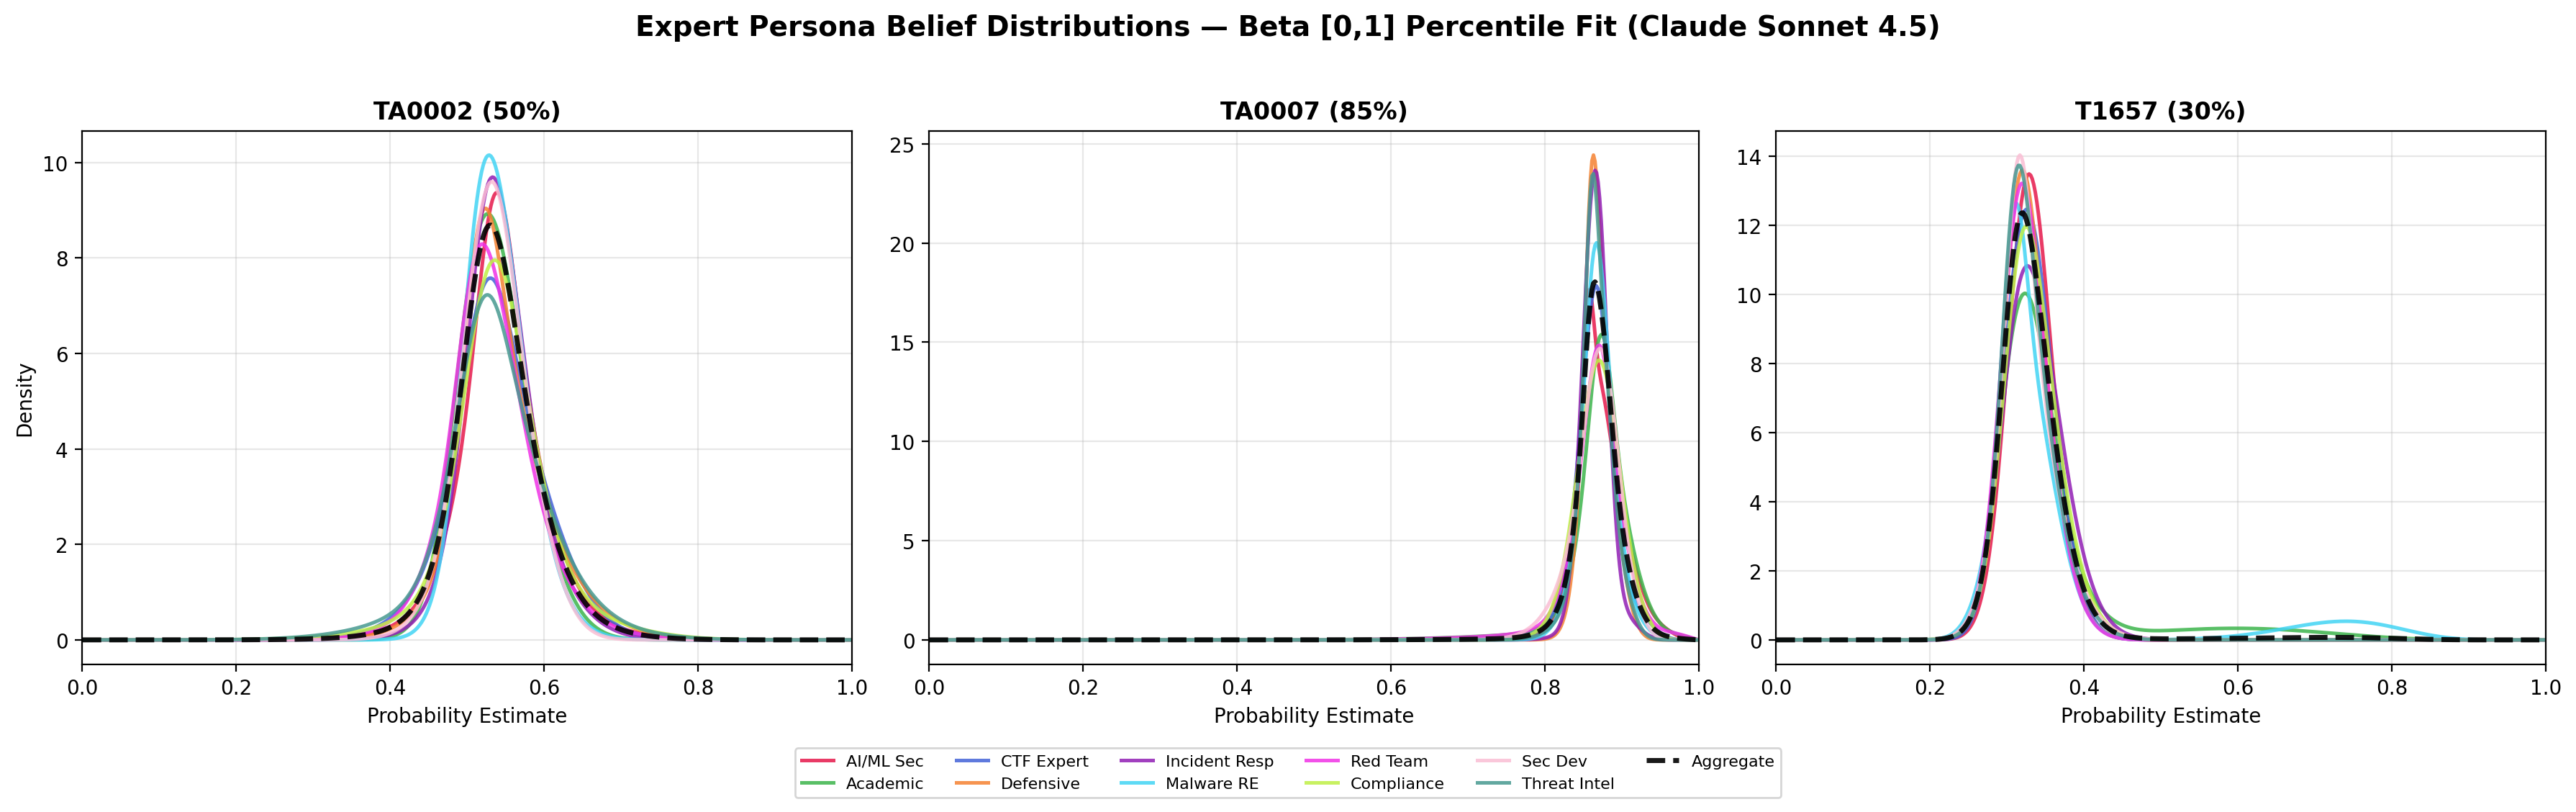
\includegraphics[width=0.85\textwidth]{figures/beta_persona_distributions_percentile_week3.png}
  \caption{Persona belief distributions for Claude Sonnet 4.5 across three attack steps. Curves overlap strongly within each step, consistent with limited persona-driven separation. At extreme baselines (30\% and 85\%), distributions become narrower, reflecting reduced uncertainty near boundaries.}
  \label{fig:persona_dist}
\end{figure}

\begin{figure}[htbp]
  \centering
  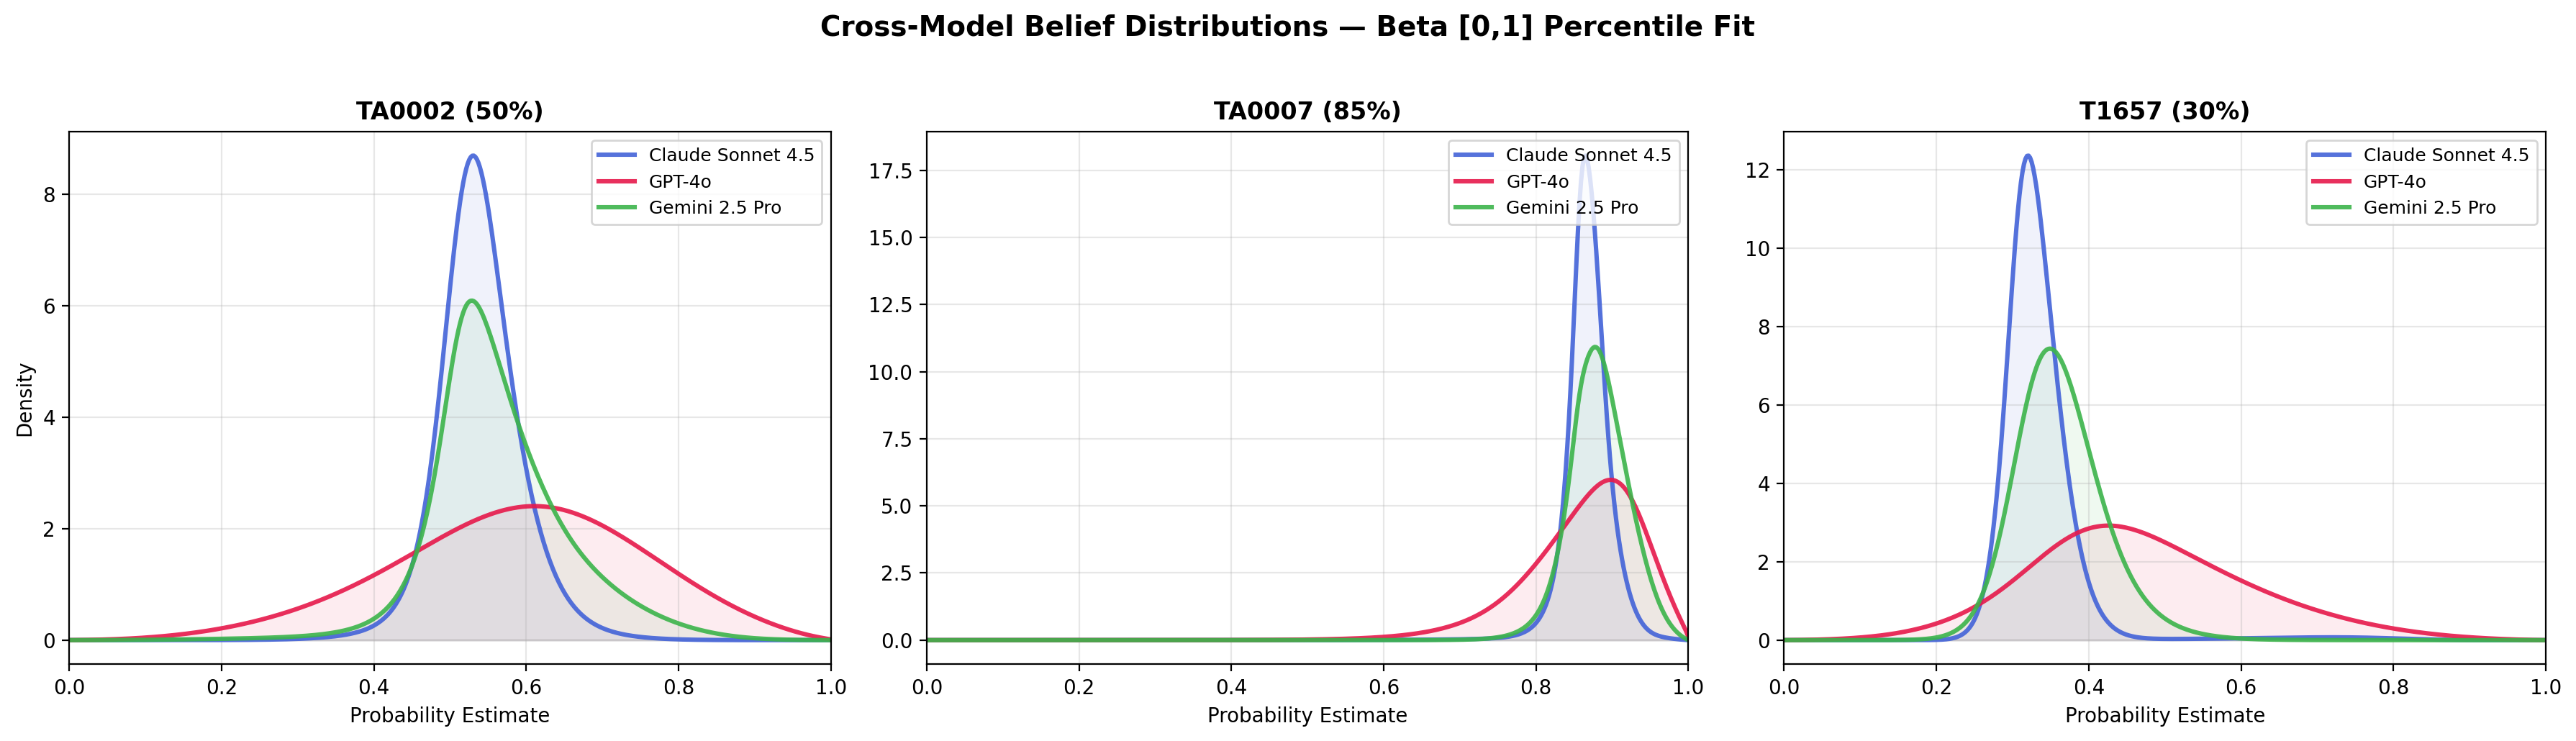
\includegraphics[width=0.85\textwidth]{figures/beta_cross_model_distributions_percentile_week3.png}
  \caption{Cross-model belief distributions show clear separation in location and spread across all three attack steps, consistent with larger model-level variance. Model differences persist across all tested baseline levels.}
  \label{fig:model_dist}
\end{figure}

\begin{figure}[htbp]
  \centering
  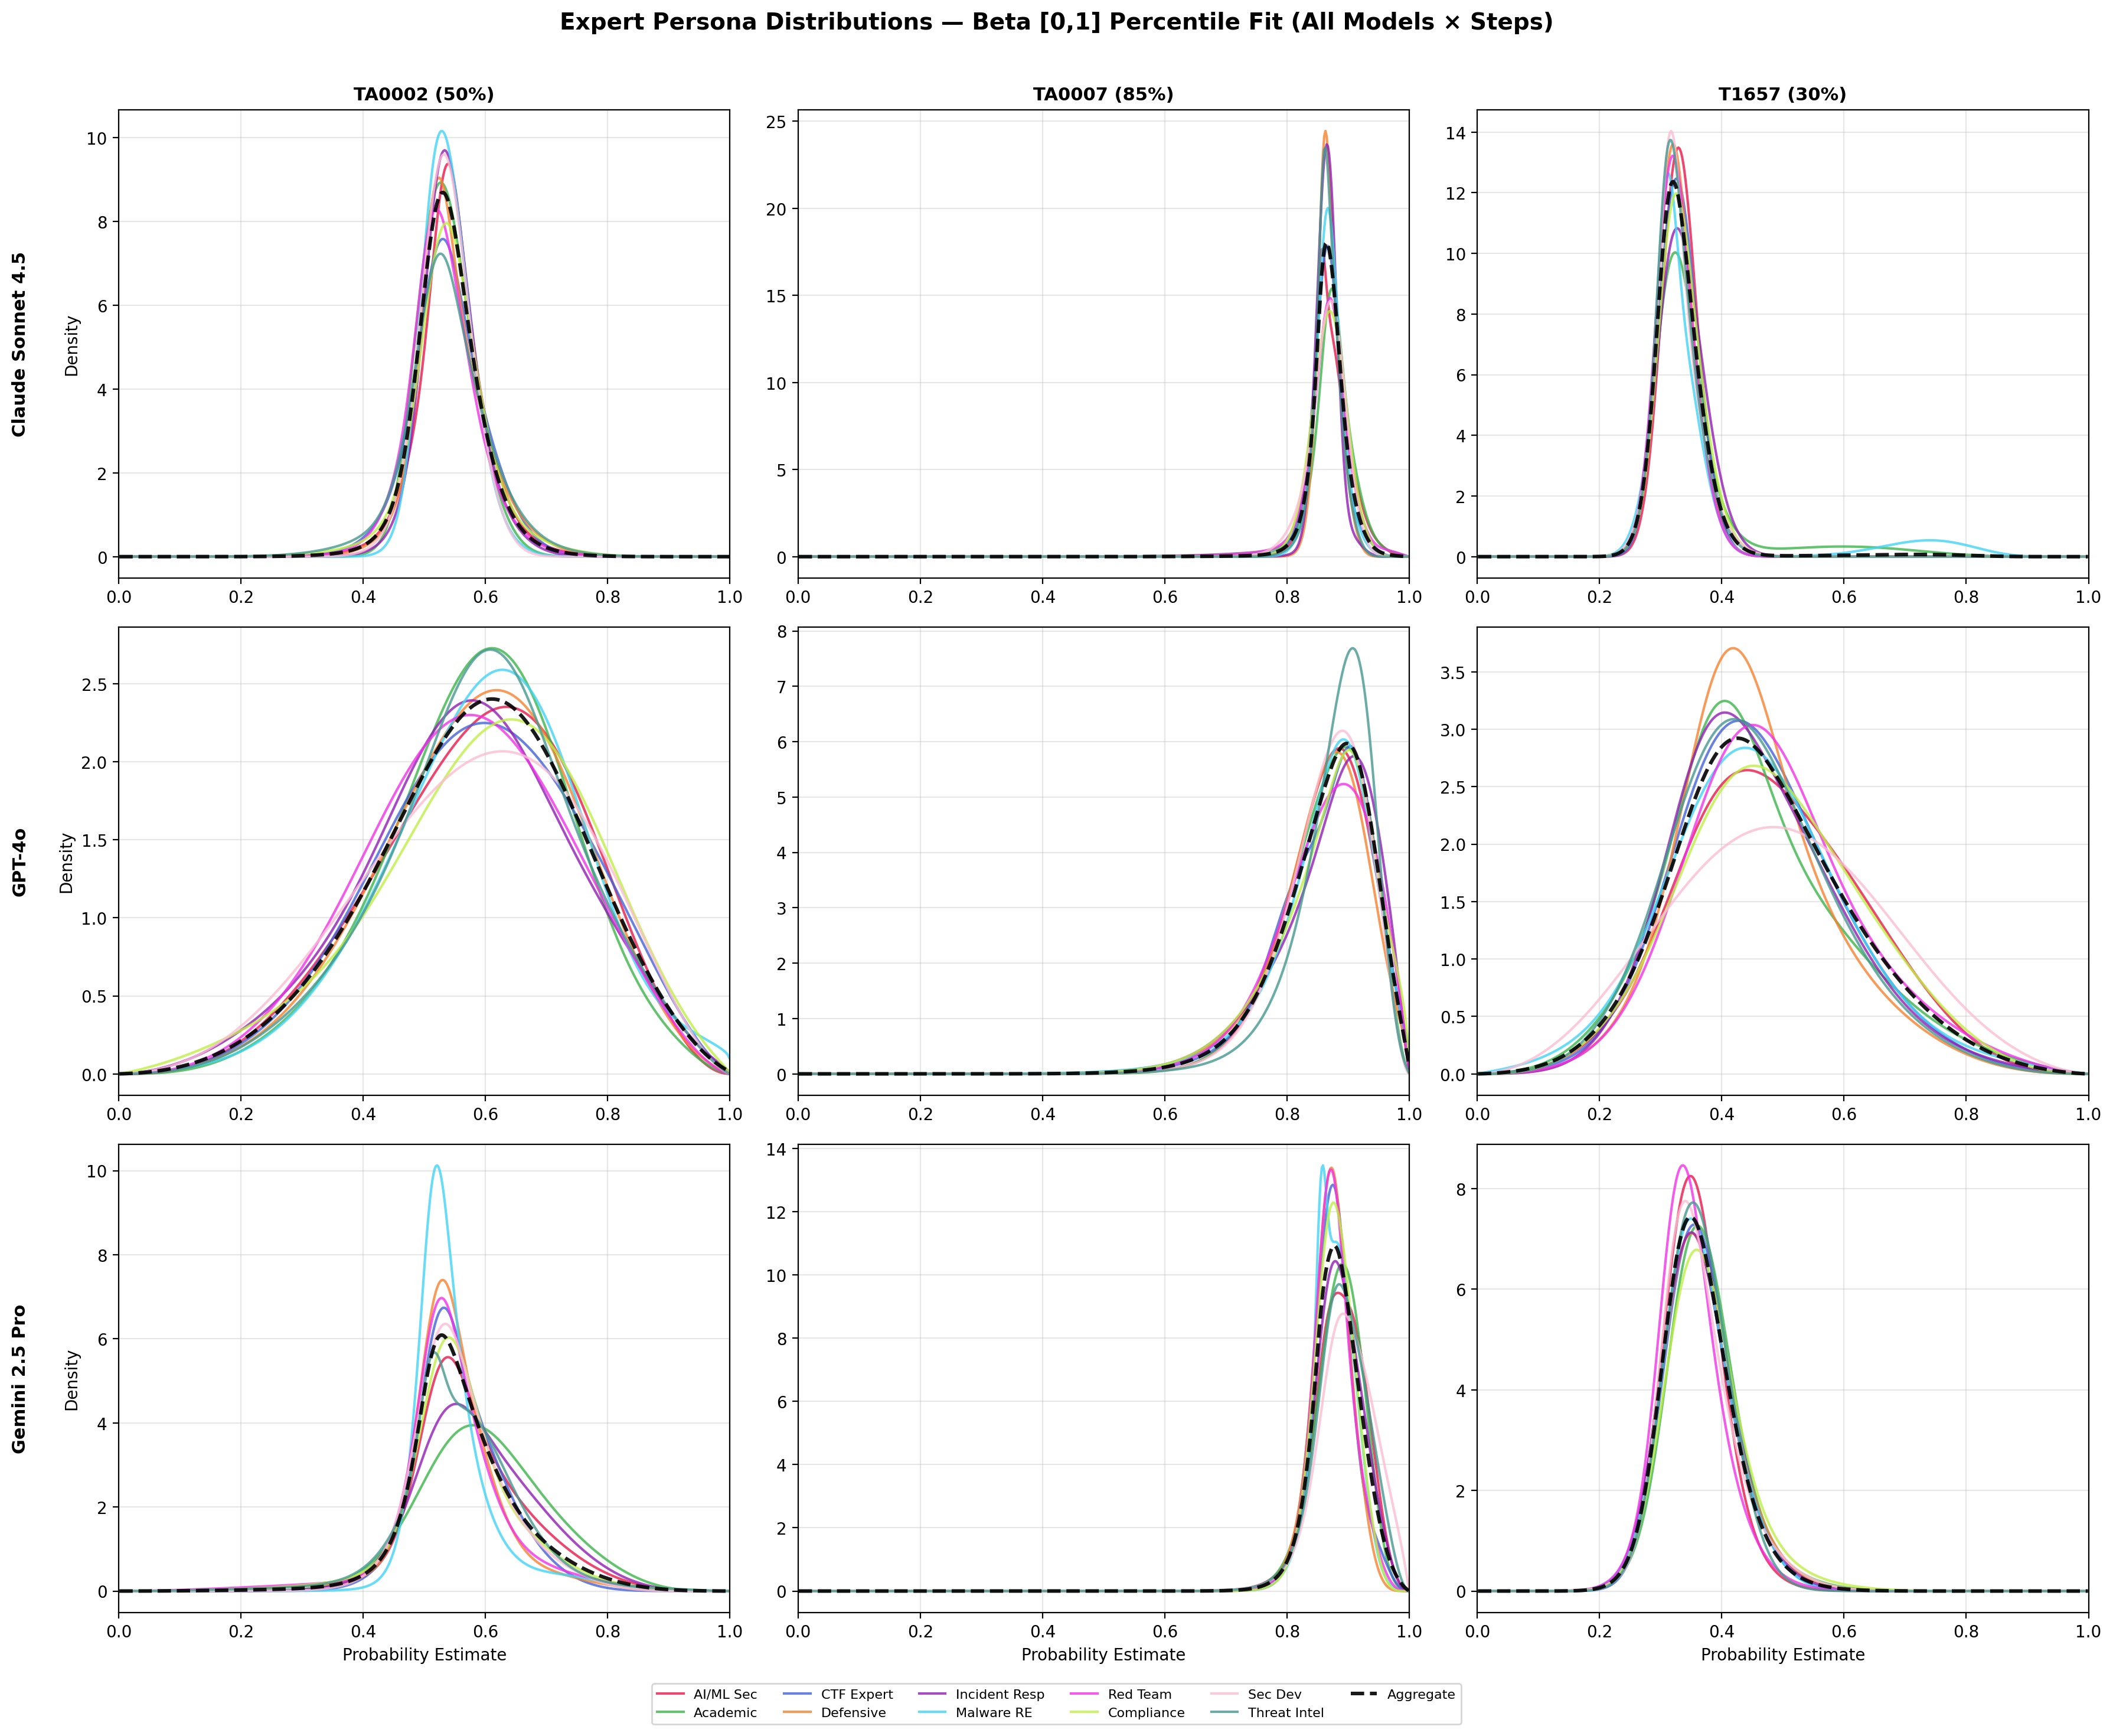
\includegraphics[width=\textwidth]{figures/beta_full_distribution_grid_percentile_week3.png}
  \caption{Full grid across models (rows) and attack steps (columns). Within-cell persona clustering is tighter than between-model shifts. Across rows (same step, different models), entire clusters shift in location and width.}
  \label{fig:full_grid}
\end{figure}

\FloatBarrier

\subsection{Strong Baseline Anchoring Effects}

\textbf{Research question:} Do LLMs anchor heavily to provided baseline probabilities, and does this pattern differ between bounded (probability) and unbounded (quantity) estimates?

\textbf{Experimental design:} Baseline swept from 10\% to 90\% in 10\% increments. Single persona (AI/ML Security Researcher), Claude Sonnet 4.6, 10 runs per baseline. Two experiments conducted:
\begin{enumerate}
\item Probability estimates: TA0002 (Execution step), Imaginairy benchmark
\item Quantity estimates: Scenario-level number of actors (unbounded integer), same benchmark
\end{enumerate}
Confidence interval wording removed from prompts to isolate baseline anchoring effect. All other prompt components held constant.

\textbf{Results:} Both probability and quantity estimates showed strong linear relationships with baseline values (Figure~\ref{fig:baseline_uplift} and Figure~\ref{fig:numactors_uplift}). For probability estimates, the relationship was approximately linear with evidence of ceiling effects at high baselines (reduced uplift approaching 100\%). For quantity estimates, the linear relationship persisted without comparable ceiling effects, consistent with the unbounded nature of the estimate.

This pattern indicates strong anchoring to provided baselines for both estimate types. The approximately linear relationship suggests LLMs may be applying relatively constant additive or multiplicative adjustments to baselines rather than reasoning independently about true probabilities. However, the presence of ceiling effects for probabilities demonstrates some awareness of the bounded constraint.

\begin{figure}[htbp]
  \centering
  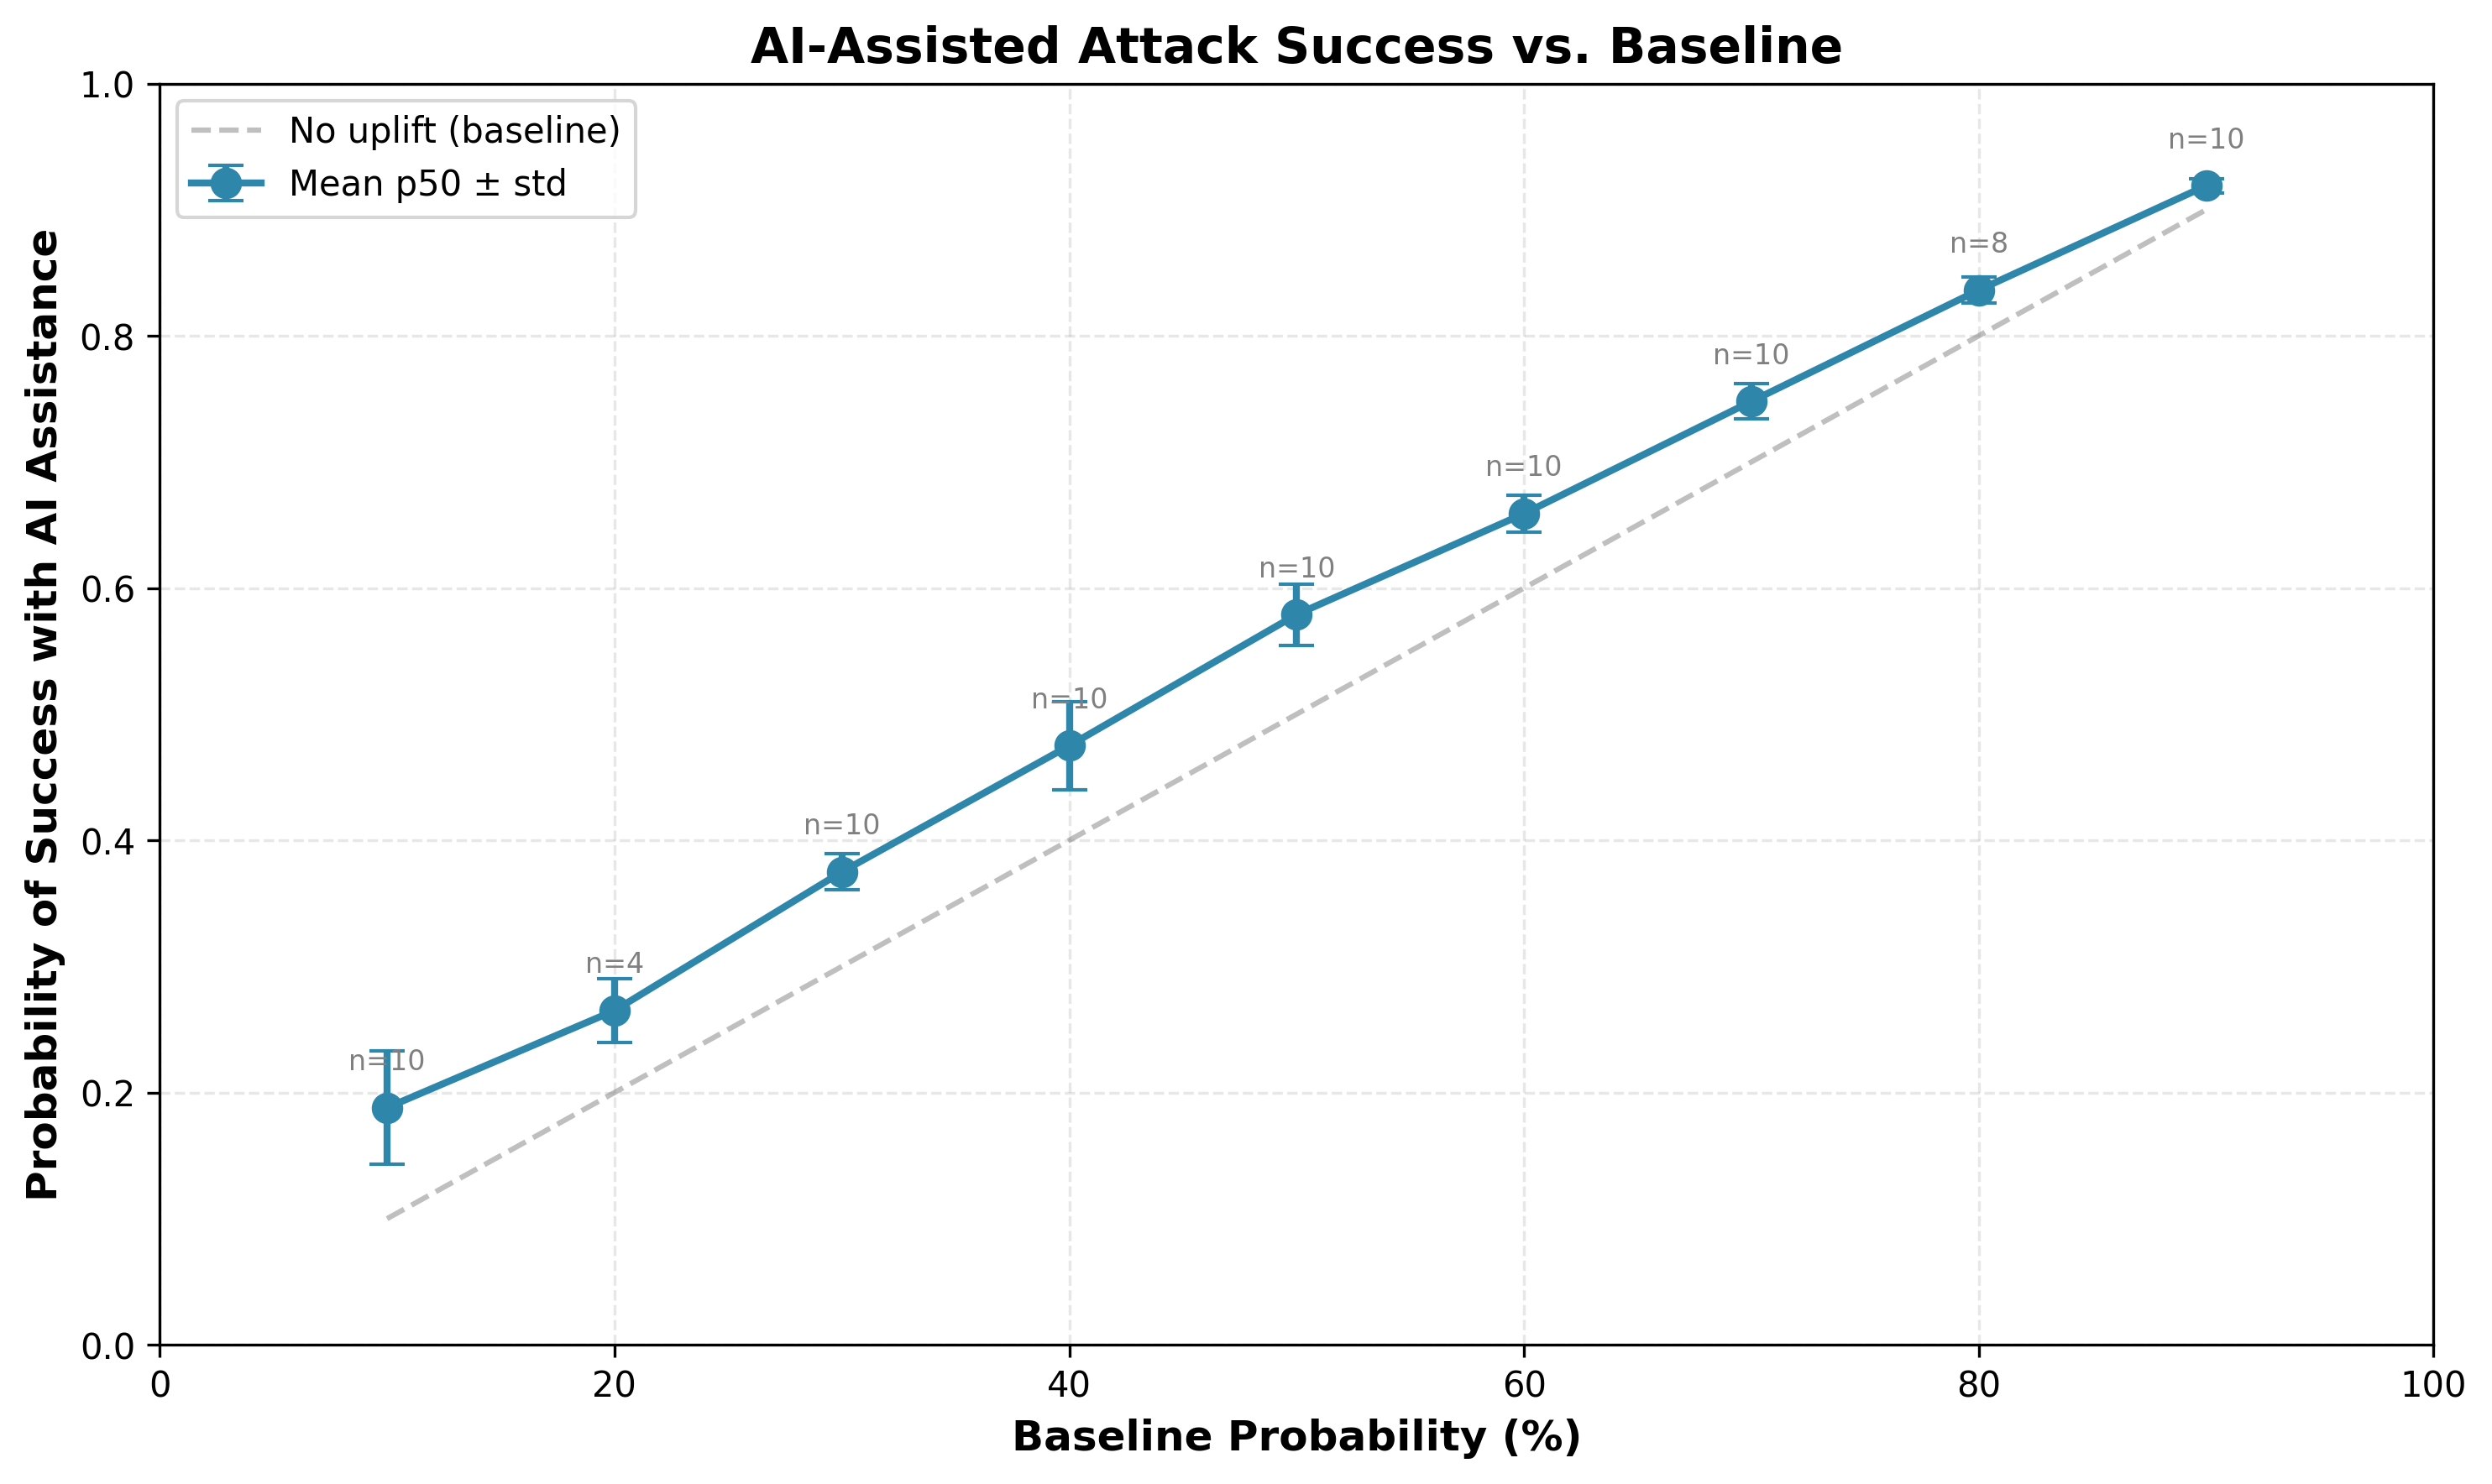
\includegraphics[width=0.75\textwidth]{figures/baseline_uplift_plot_week5.png}
  \caption{Median elicited probability vs. baseline for TA0002 (Execution step). Baseline varied 10\%--90\%, Claude Sonnet 4.6, single persona (AI/ML Security Researcher), 10 runs per baseline, Imaginairy benchmark. Error bars show interquartile range across runs. Approximately linear relationship with ceiling effect at high baselines.}
  \label{fig:baseline_uplift}
\end{figure}

\begin{figure}[htbp]
  \centering
  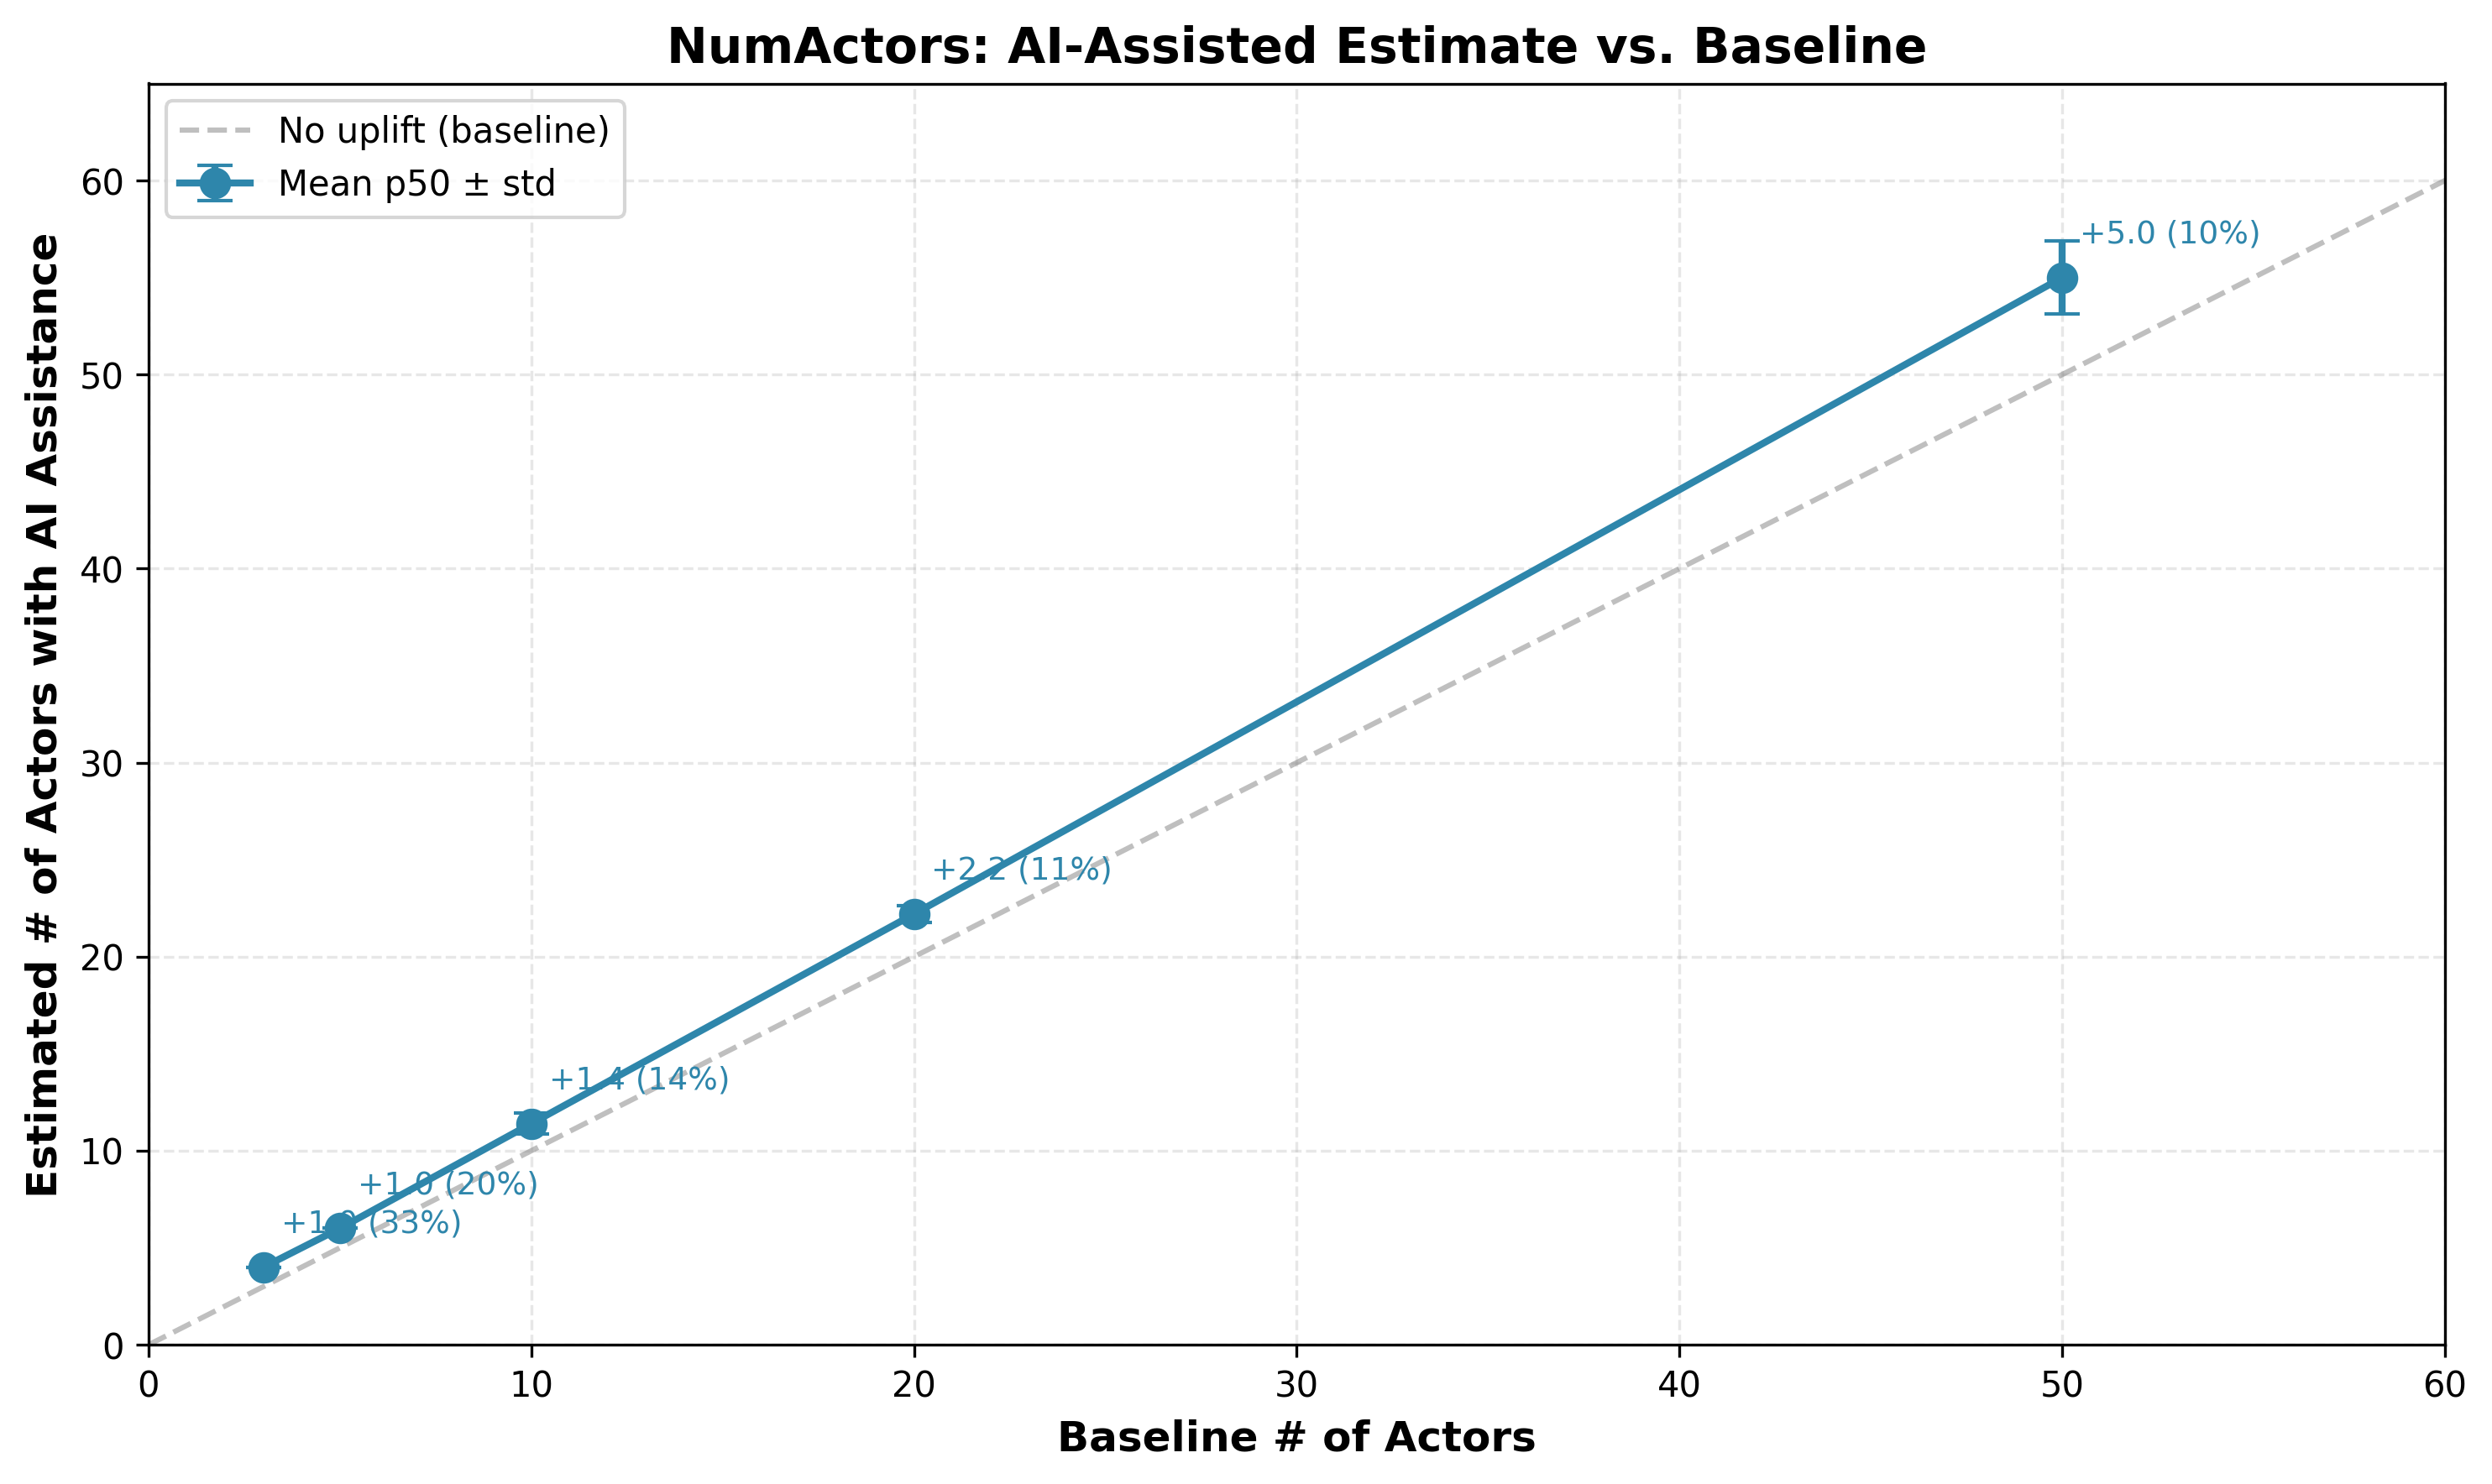
\includegraphics[width=0.75\textwidth]{figures/numactors_baseline_uplift_plot.png}
  \caption{Elicited number of actors vs. baseline (scenario-level estimate). Claude Sonnet 4.6, single persona, Imaginairy benchmark, 10 runs per baseline. The relationship is approximately linear without ceiling effects, consistent with baseline anchoring in unbounded quantity estimates.}
  \label{fig:numactors_uplift}
\end{figure}

\FloatBarrier

\subsection{Prompt Sensitivity Varies by Component}

\textbf{Research question:} Which prompt components most strongly influence forecast distributions and variance?

\textbf{Experimental design:} Seven prompt conditions tested against full control prompt. Single expert persona (AI/ML Security Researcher), Claude Sonnet 4.5, 10 runs per condition. Attack step: TA0002 (Execution, 50\% baseline), Imaginairy benchmark. Conditions:

\begin{enumerate}
\item \textbf{Control:} Full prompt (615 words)
\item \textbf{no\_ci:} Removed uncertainty range (5th/95th percentile: "20\%--90\%") from baseline
\item \textbf{no\_baseline:} Removed point estimate ("50\% chance of success") from baseline
\item \textbf{no\_baseline\_no\_ci:} Removed entire baseline statement
\item \textbf{skip\_analysis:} Removed detailed capability analysis instructions (4-section breakdown)
\item \textbf{trim\_reasoning:} Removed 3-phase reasoning scaffold
\item \textbf{trim\_all:} Removed capability analysis + reasoning scaffold + technical analysis output ($\sim$100 words)
\end{enumerate}

Distributional shift measured using W$_1$ distance from control condition. Variance measured as squared W$_2$ distance, reported as multiplier of control variance.

\textbf{Results:} Removing the baseline produced the largest distributional shifts (Table~\ref{tab:prompt_sensitivity}, Figure~\ref{fig:prompt_sensitivity}). The no\_baseline condition showed W$_1$ = 0.154 with 18.1$\times$ control variance, while no\_baseline\_no\_ci showed W$_1$ = 0.230 with 12.3$\times$ control variance. In contrast, removing confidence interval wording alone had minimal impact (W$_1$ = 0.013, variance 0.36$\times$ control).

Surprisingly, trimming reasoning scaffolds and capability analysis produced small distributional shifts (trim\_reasoning: W$_1$ = 0.011, trim\_all: W$_1$ = 0.016) and substantially \emph{reduced} variance (0.30$\times$ and 0.07$\times$ control respectively). This suggests the model converges to more consistent estimates under shorter, more direct prompts. The trim\_all condition reduced prompt length from 615 words to approximately 100 words while maintaining similar central estimates with dramatically reduced variance.

\begin{table}[htbp]
\centering
\caption{Prompt sensitivity results. W$_1$ distance measures distributional shift from control; variance shown as multiplier of control-condition variance. Removing baseline produces largest shifts and variance increases. Trimming reasoning scaffolds reduces variance.}
\label{tab:prompt_sensitivity}
\begin{tabular}{lcc}
\toprule
\textbf{Condition} & \textbf{W$_1$ Distance} & \textbf{W$^2$ Variance ($\times$Control)} \\
\midrule
Control (full prompt, 615 words) & --- & 1.00$\times$ \\
no\_ci & 0.013 & 0.36$\times$ \\
no\_baseline & 0.154 & 18.1$\times$ \\
no\_baseline\_no\_ci & 0.230 & 12.3$\times$ \\
skip\_analysis & 0.041 & 0.78$\times$ \\
trim\_reasoning & 0.011 & 0.30$\times$ \\
trim\_all ($\sim$100 words) & 0.016 & 0.07$\times$ \\
\bottomrule
\end{tabular}
\end{table}

\begin{figure}[htbp]
  \centering
  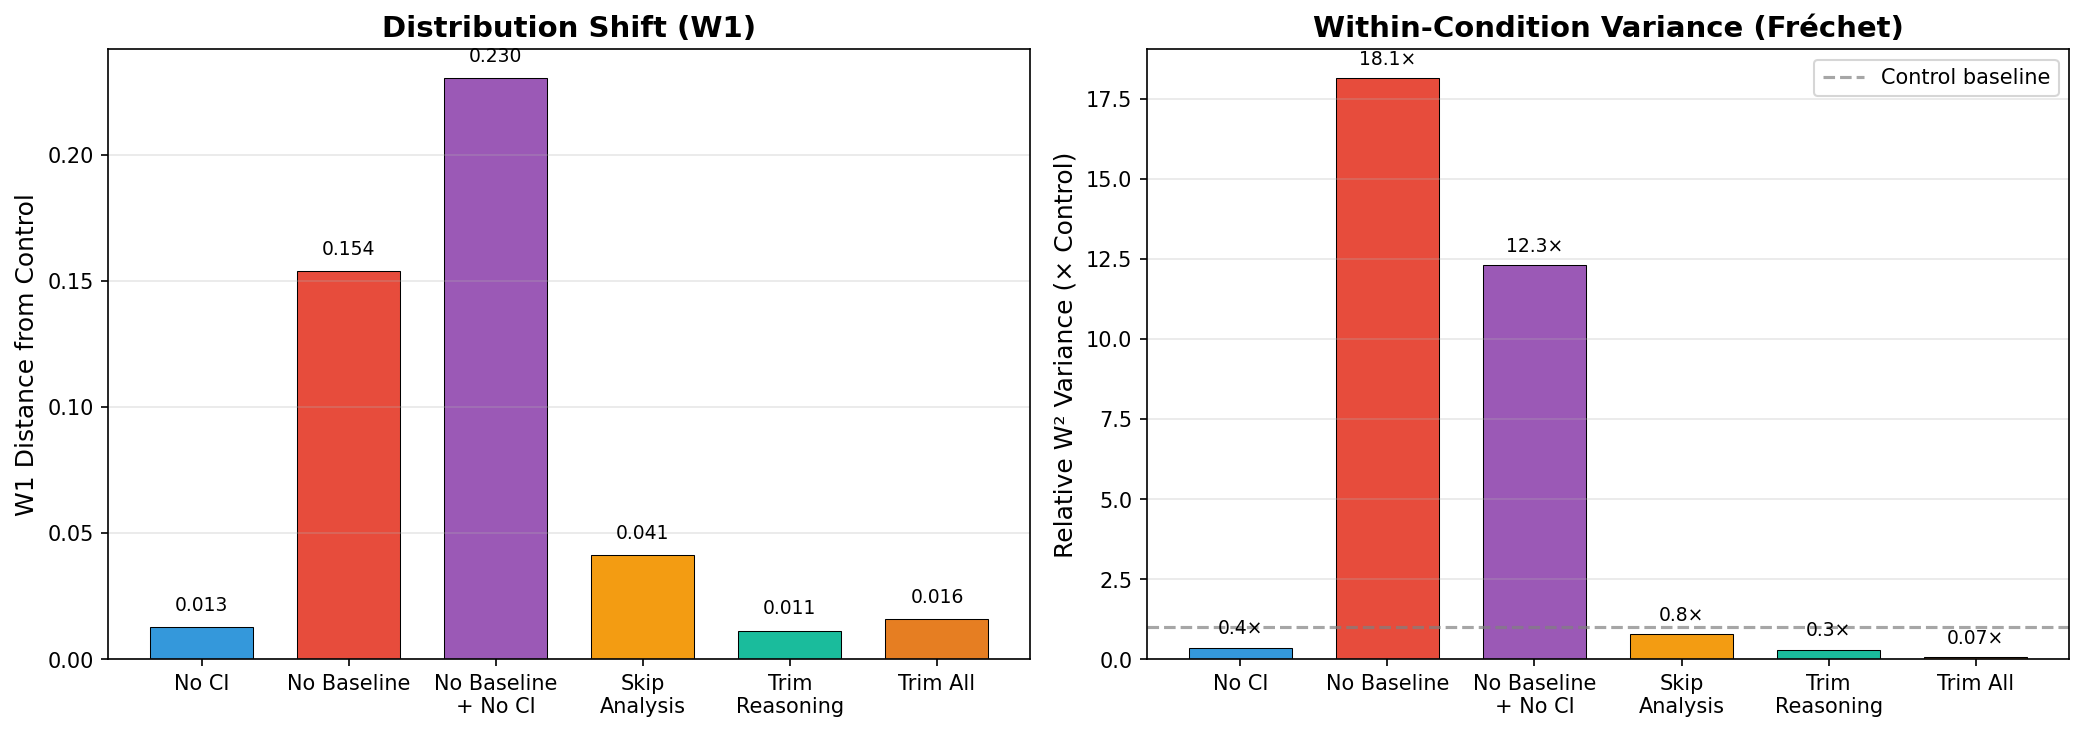
\includegraphics[width=0.8\textwidth]{figures/w1_chart (1)_week5.png}
  \caption{W$_1$ distance to control across seven prompt conditions. Baseline-removal conditions shift distributions most substantially. Trimming reasoning scaffolds (trim\_reasoning, trim\_all) produces smallest shifts and dramatically reduced variance, suggesting convergence under shorter prompts.}
  \label{fig:prompt_sensitivity}
\end{figure}

\FloatBarrier

\subsection{Quantities Show Higher Variance Than Probabilities}

\textbf{Research question:} Do quantity estimates (number of actors) show higher expert disagreement than probability estimates, mirroring patterns observed in human expert elicitation?

\textbf{Experimental design:} Within-model comparison of coefficient of variation (CV) across estimate types. Three models tested (Claude Sonnet 4.5, GPT-4o, Gemini 2.5 Pro), 10 personas, 10 runs per persona-model combination.
\begin{itemize}
\item Probability estimates: Three attack steps (TA0002 50\%, TA0007 85\%, T1657 30\%), Imaginairy benchmark
\item Quantity estimates: Scenario-level number of actors, same benchmark context
\end{itemize}

CV computed from median values (p50) across runs for each persona, then averaged across personas. For probability estimates, CV averaged across the three attack steps.

\textbf{Results:} All three models showed higher variance for quantity estimates than probability estimates (Table~\ref{tab:quantity_variance}). GPT-4o: 4.7\% vs 1.9\% (2.5$\times$ ratio), Gemini: 6.0\% vs 2.2\% (2.7$\times$ ratio), Claude: 6.2\% vs 1.7\% (3.6$\times$ ratio).

This pattern is consistent with human expert elicitation, where quantity estimates showed substantially higher disagreement (CV 65--89\%) than probability estimates. However, LLM disagreement on quantities was notably lower than human disagreement (LLM: 12--19\% CV for number of actors vs human: 65--89\% CV), suggesting either greater consistency or potential anchoring effects in LLM quantity estimates.

\textbf{Note on model variance:} This finding held despite model choice being the dominant variance source. Fréchet ANOVA on quantity estimates showed model ICC\_F = 24\% vs persona ICC\_F = 9\%, a 2.6$\times$ ratio consistent with the 3--5$\times$ ratio observed for probability estimates (model ICC\_F = 58\%, persona ICC\_F = 12\%).

\begin{table}[htbp]
\centering
\caption{Coefficient of variation comparison across estimate types. All models show higher variance for quantity estimates (number of actors) than probability estimates, consistent with human expert patterns but with lower absolute disagreement levels.}
\label{tab:quantity_variance}
\begin{tabular}{lccc}
\toprule
\textbf{Model} & \textbf{Quantity CV} & \textbf{Probability CV} & \textbf{Ratio} \\
\midrule
GPT-4o & 4.7\% & 1.9\% & 2.5$\times$ \\
Gemini 2.5 Pro & 6.0\% & 2.2\% & 2.7$\times$ \\
Claude Sonnet 4.5 & 6.2\% & 1.7\% & 3.6$\times$ \\
\bottomrule
\end{tabular}
\end{table}

\FloatBarrier

% ============================================================================
% LIMITATIONS AND DISCUSSION
% ============================================================================
\section{Limitations and Open Questions}

\subsection{Generalization}

Most experiments used a small set of attack scenarios (primarily TA0001, TA0002, TA0007, T1657) and benchmark tasks (primarily Imaginairy, with limited testing on MLFlow0 and cURL). Findings may not generalize to other MITRE ATT\&CK steps, more complex multi-step scenarios, or substantially different benchmark structures. The prompt trimming result is particularly surprising and requires extensive replication across different tasks, benchmarks, and models before being taken seriously for production use.

Additionally, all experiments used a ransomware scenario targeting a large enterprise. Different threat scenarios (e.g., state-sponsored espionage, insider threats) or different target profiles may show different patterns of model behavior and variance.

\subsection{Ground Truth Validation}

The baseline anchoring finding raises critical questions about whether LLMs are genuinely reasoning about capability transfer or primarily manipulating provided anchors. The approximately linear relationship between baseline and output for both probability and quantity estimates suggests potential over-reliance on anchoring rather than independent assessment.

Without ground truth for many scenarios, it is difficult to assess whether model outputs reflect genuine expertise or learned patterns from training data. The memorization concerns raised in prior work~\cite{leung2024memorization} suggest that LLMs may retrieve benchmark-related information from training rather than reasoning about capability transfer. Published benchmark scores are present in training data, making it difficult to distinguish between retrieval and reasoning.

\subsection{Methodological Limitations}

Several methodological choices warrant discussion:

\textbf{Fitting assumptions:} All distributional analyses used Beta distributions fit to three quantiles (p25, p50, p75). This assumption may not be appropriate for all elicitation patterns, particularly those with irregular shapes or multimodality. For quantity estimates, we assumed bounded support and fit PERT distributions, which may not suit unbounded integers well. Alternative approaches (e.g., lognormal for quantities) should be explored.

\textbf{Variance comparison:} Comparing variance between probability and quantity estimates required averaging CVs across different baselines (30\%, 50\%, 85\%) for probabilities, which may not be directly comparable due to ceiling/floor effects. However, the 2.5--3.6$\times$ ratio is large enough that the conclusion likely holds despite this limitation.

\textbf{Statistical power:} Within-model persona comparisons used 10 runs per persona, which may have limited power to detect small but meaningful persona effects. However, the consistency of null results across multiple models and attack steps, combined with the much larger effects observed for model choice, suggests persona effects are genuinely small rather than merely undetectable.

\subsection{Implications for LLM-Based Forecasting}

The dominance of model variance over persona variance has important implications for forecasting system design. If persona choice has minimal impact, resources spent on careful persona design and selection may be better directed toward model selection, prompt engineering for consistency, or ensemble methods across models.

The strong baseline anchoring effects suggest that baseline values must be chosen very carefully, as they substantially influence outputs. This raises questions about whether LLMs should be provided with baselines at all, or whether alternative elicitation approaches that avoid anchoring would be preferable. However, the baseline removal experiments showed dramatically increased variance, suggesting baselines serve an important variance-reduction function even if they bias estimates.

The surprising prompt trimming results suggest potential for substantial efficiency gains, but require much more extensive validation before deployment. If the trim\_all condition's performance holds across diverse tasks and models, reducing prompt length by 80\% while maintaining or improving consistency would have significant practical value.

% ============================================================================
% NEXT STEPS
% ============================================================================
\section{Next Steps}

\subsection{Expanded Experimental Coverage}

\textbf{Prompt trimming validation:} Replicate trim\_reasoning and trim\_all conditions across diverse attack steps, benchmark tasks, and models. If results hold, conduct systematic ablation to identify minimal sufficient prompt components.

\textbf{Baseline mechanisms:} Conduct experiments to distinguish between additive, multiplicative, and other anchoring patterns. Test whether providing baselines as ranges rather than point estimates reduces anchoring while maintaining variance reduction.

\textbf{Difficulty effects:} Systematically vary benchmark difficulty (using LLM-estimated difficulty scores) to test whether forecast variance and bias change with task difficulty, as observed in some human expert studies.

\subsection{Ground Truth Development}

\textbf{Intra-benchmark validation:} Develop ground truth using conditional probabilities within benchmark suites. For example, using LiveBench data (195 models, multiple domains, per-task scores): ask LLMs "Model X solved task A, what is P(solves task B)?" Compare against empirical rates: $\frac{\#\{\text{models solving both A and B}\}}{\#\{\text{models solving A}\}}$.

This approach leverages published model performance data to create scalable ground truth without requiring human expert elicitation or expensive model evaluations.

\textbf{Cross-benchmark correlation:} Extend intra-benchmark approach to cross-benchmark predictions. Test whether LLMs can predict performance on cybersecurity benchmarks (Cybench, BountyBench) conditional on performance on coding benchmarks (HumanEval, MBPP) or general reasoning benchmarks (MMLU, GPQA).

\subsection{Ensemble and Aggregation Methods}

Given that model choice explains 48--69\% of variance while persona choice explains $\leq$25\%, investigate ensemble methods that combine forecasts across models rather than personas. Test whether simple averaging, variance-weighted averaging, or more sophisticated aggregation improves forecast accuracy and calibration.

% ============================================================================
% BIBLIOGRAPHY
% ============================================================================
\bibliographystyle{plain}
\bibliography{references}

\end{document}
